\documentclass[a4paper, 11pt]{article}           %{{{1
% basic packages                                  {{{2
\usepackage[T1]{fontenc}
\usepackage[scaled=0.975]{helvet}
\usepackage[utf8]{inputenc}
\usepackage{amsmath}
\usepackage{lastpage}
\usepackage{graphicx}
\usepackage{amsfonts}
\usepackage{variations}
\usepackage{pgf,tikz}           % dessin
\usepackage{mathrsfs}
\usetikzlibrary{arrows}
\usepackage{pgfkeys}        % fenetrage des plot TikZ
\usepackage{yhmath}         % arc au dessus des lettres
\usepackage{calc}           % calcul de longueur
\usepackage{variations}     % tableau de variations
\usepackage{multicol}
\usepackage{enumitem}
\usepackage{fancyhdr}                                                           % configuration ci-dessous
% ==== EDITION
% marges {{{3
\addtolength{\voffset}{-1.8cm}
\addtolength{\textheight}{4cm}
\addtolength{\hoffset}{-2.5cm}
\addtolength{\textwidth}{4cm}
\addtolength{\headsep}{-0.5cm}
%}}}
% fancyhdr {{{3
\setlength{\headheight}{14.00pt}                                                %
\pagestyle{fancy}                                                               % Numérotation des pages
\renewcommand\footrulewidth{1pt}                                                %
\renewcommand\headrulewidth{1pt}                                                %
\fancyhead[L]{2nd SN}
\fancyhead[C]{PWM, LED RGB et potentiomètre}
\fancyhead[R]{arduino}
\fancyfoot[L]{v 1.1 - JB}
\fancyfoot[C]{\textbf{Audiovisuel professionnel}}   %
\fancyfoot[R]{\thepage/\pageref{LastPage}}
% }}}
% ==== PROGRAMMATION
\usepackage{xcolor}                                                             %
\usepackage{tcolorbox}                                                          % encadrement texte
\usepackage{listings}                                                           %
% listings                                        {{{3
\definecolor{mygreen}{rgb}{0,0.6,0}
\definecolor{mygray}{rgb}{0.5,0.5,0.5}
\definecolor{mymauve}{rgb}{0.58,0,0.82}
\definecolor{deepblue}{rgb}{0,0,0.5}
\definecolor{deepred}{rgb}{0.6,0,0}
\definecolor{deepgreen}{rgb}{0,0.5,0}
\lstset{%
% backgroundcolor=\color{white},   % choose the background color; you must add \usepackage{color} or \usepackage{xcolor}; should come as last argument
  basicstyle=\footnotesize,        % the size of the fonts that are used for the code
% breakatwhitespace=false,         % sets if automatic breaks should only happen at whitespace
% breaklines=true,                 % sets automatic line breaking
% captionpos=b,                    % sets the caption-position to bottom
  commentstyle=\color{mygreen},    % comment style
% deletekeywords={type},           % if you want to delete keywords from the given language
% emph={},                         % Custom highlighting
% emphstyle=\ttb\color{deepred}    % Custom highlighting style
% escapeinside={\%*}{*)},          % if you want to add LaTeX within your code
% extendedchars=true,              % lets you use non-ASCII characters; for 8-bits encodings only, does not work with UTF-8
  frame=shadowbox,                 % adds a frame around the code {single, shadowbox}
% keepspaces=true,                 % keeps spaces in text, useful for keeping indentation of code (possibly needs columns=flexible)
  keywordstyle=\color{blue},       % keyword style
  language=C,                      % the language of the code {Python, C}
% morekeywords={*,...},            % if you want to add more keywords to the set
  numbers=left,                    % numbers = (none, left, right)
% numbersep=5pt,                   % how far the line-numbers are from the code
% numberstyle=\tiny\color{mygray}, % the style that is used for the line-numbers
% otherkeywords={self},            % Add keywords here
% rulecolor=\color{black},         % if not set, the frame-color may be changed on line-breaks within not-black text (e.g. comments (green here))
  rulesepcolor=\color{gray}        % shadowbox color
% showspaces=false,                % show spaces everywhere adding particular underscores; it overrides 'showstringspaces'
% showstringspaces=false,          % underline spaces within strings only
% showtabs=false,                  % show tabs within strings adding particular underscores
% stepnumber=1,                    % the step between two line-numbers. If it's 1, each line will be numbered
% stringstyle=\color{mymauve},     % string literal style
% tabsize=4,                       % sets default tabsize to 2 spaces
% title=\lstname                   % show the filename of files included with \lstinputlisting; also try caption instead of title
}
%}}}
%}}}

% Compteurs:                                     {{{2
\addtocounter{page}{0}
\newcounter{Q}
\newcounter{exoNB}
%}}}

% Longueur:                                      {{{2
\newlength{\longueurA}
\newlength{\longueurB}
\setlength{\parindent}{0pt}
\setlength{\parskip}{2pt}
\renewcommand{\baselinestretch}{1}
%}}}

% newcommand                                     {{{2
\newcommand{\objectif}[1]{\textsc{\Huge #1} }
\newcommand{\partie}[1]{\textsc{\huge #1} }
\newcommand{\question}{\stepcounter{Q} $\boxed{\arabic{Q}}$ }
\newcommand{\ligne}{\underline{\hspace{ \textwidth}} }
\newcommand{\exo}[1]{\stepcounter{exoNB}\textsc{\Large Exercice \arabic{exoNB} -- #1} }
\newcommand{\EXO}[2]{\stepcounter{exoNB}\textsc{\Large Exercice \arabic{exoNB} -- #1} \hfill \textbf{#2 points}}
\newcommand{\pb}[1] {\stepcounter{exoNB}\textsc{\Large Problème \arabic{exoNB} -- #1} }
\newcommand{\PB}[2] {\stepcounter{exoNB}\textsc{\Large Problème \arabic{exoNB} -- #1} \hfill \textbf{#2 points}}
\newcommand{\reponse}{
  \par\nobreak
  \noindent\rule{0pt}{1.5\baselineskip}% Provides a larger gap between the preceding paragraph and the dots
  {\noindent\makebox[\linewidth]{\dotfill}\endgraf}% ... dotted lines ...
% \bigskip% Gap between dots and next paragraph
  }
%}}}

% Divers                                          {{{2
% listings                                        {{{3
%\definecolor{mygreen}{rgb}{0,0.6,0}
%\definecolor{mygray}{rgb}{0.5,0.5,0.5}
%\definecolor{mymauve}{rgb}{0.58,0,0.82}
%\definecolor{deepblue}{rgb}{0,0,0.5}
%\definecolor{deepred}{rgb}{0.6,0,0}
%\definecolor{deepgreen}{rgb}{0,0.5,0}
%\lstset{%
%        backgroundcolor=\color{white},   % choose the background color; you must add \usepackage{color} or \usepackage{xcolor}; should come as last argument
%        basicstyle=\footnotesize,        % the size of the fonts that are used for the code
%        breakatwhitespace=false,         % sets if automatic breaks should only happen at whitespace
%        breaklines=true,                 % sets automatic line breaking
%        captionpos=b,                    % sets the caption-position to bottom
%        commentstyle=\color{mygreen},    % comment style
%        deletekeywords={...},            % if you want to delete keywords from the given language
%        escapeinside={\%*}{*)},          % if you want to add LaTeX within your code
%        extendedchars=true,              % lets you use non-ASCII characters; for 8-bits encodings only, does not work with UTF-8
%        frame=single,                    % adds a frame around the code
%        keepspaces=true,                 % keeps spaces in text, useful for keeping indentation of code (possibly needs columns=flexible)
%        keywordstyle=\color{blue},       % keyword style
%        morekeywords={*,...},            % if you want to add more keywords to the set
%        numbers=left,                    % where to put the line-numbers; possible values are (none, left, right)
%        numbersep=5pt,                   % how far the line-numbers are from the code
%        numberstyle=\tiny\color{mygray}, % the style that is used for the line-numbers
%        rulecolor=\color{black},         % if not set, the frame-color may be changed on line-breaks within not-black text (e.g. comments (green here))
%        showspaces=false,                % show spaces everywhere adding particular underscores; it overrides 'showstringspaces'
%        showstringspaces=false,          % underline spaces within strings only
%        showtabs=false,                  % show tabs within strings adding particular underscores
%        stepnumber=2,                    % the step between two line-numbers. If it's 1, each line will be numbered
%        stringstyle=\color{mymauve},     % string literal style
%        tabsize=4,                       % sets default tabsize to 2 spaces
%        title=\lstname                   % show the filename of files included with \lstinputlisting; also try caption instead of title
%}
%\lstset{%
%        language=Python,                 % the language of the code
%        otherkeywords={self},            % Add keywords here
%        deletekeywords={type},           % if you want to delete keywords from the given language
%        emph={},                         % Custom highlighting
%        emphstyle=\ttb\color{deepred}    % Custom highlighting style
%}
%}}}

% PRL style line                                 {{{3
\newlength{\diamondrulelength}
\setlength{\diamondrulelength}{0.6\textwidth}
\newlength{\diamondrulethickness}
\setlength{\diamondrulethickness}{2pt}
\newcommand{\diamondrule}{\begin{center}\tikz{\fill[black] (0.5\diamondrulelength,0) -- (0,0.5\diamondrulethickness) -- (-0.5\diamondrulelength,0) -- (0,-0.5\diamondrulethickness) -- cycle;}\end{center}}
%}}}

% fixed with tabular                             {{{3
\usepackage{array}
\newcolumntype{L}[1]{>{\raggedright\let\newline\\\arraybackslash\hspace{0pt}}m{#1}}
\newcolumntype{C}[1]{>{\centering\let\newline\\\arraybackslash\hspace{0pt}}m{#1}}
\newcolumntype{R}[1]{>{\raggedleft\let\newline\\\arraybackslash\hspace{0pt}}m{#1}}
%}}}

%}}}
%}}}

\begin{document}
\sffamily
\hfill Nom : {\noindent\makebox[5cm]{\dotfill}\endgraf}
\objectif{Gradateur et synthèse de couleur}\\ %{{{1

\begin{minipage}{0.46\textwidth}
Un gradateur est un système électrique destiné à faire varier la puissance délivrée à un appareil, souvent un éclairage (projecteurs de scène, par exemple). C'est donc un dispositif d'électronique de puissance qui fonctionne en faisant varier la tension et le courant de sortie. Ainsi, il modifie la puissance utile appliqué à l'appareil qu'il alimente. En électronique de puissance, on nomme l'appareil qui reçoit la puissance électrique la charge.

Un particularité du gradateur est de diminuer la puissance délivrée à la charge en comparaison d'un circuit sans gradateur. Dans les situtions réelles, ce dispositif est utilisé sur des tensions alternatives (souvent sinusoïdales) : c'est un convertisseur direct alternatif-alternatif. Ceci étant précisé, dans le cadre de ce sujet, le gradateur étudié fonctionne en courant continu.\\
\end{minipage}\hfill
\begin{minipage}{0.46\textwidth}
\begin{center}
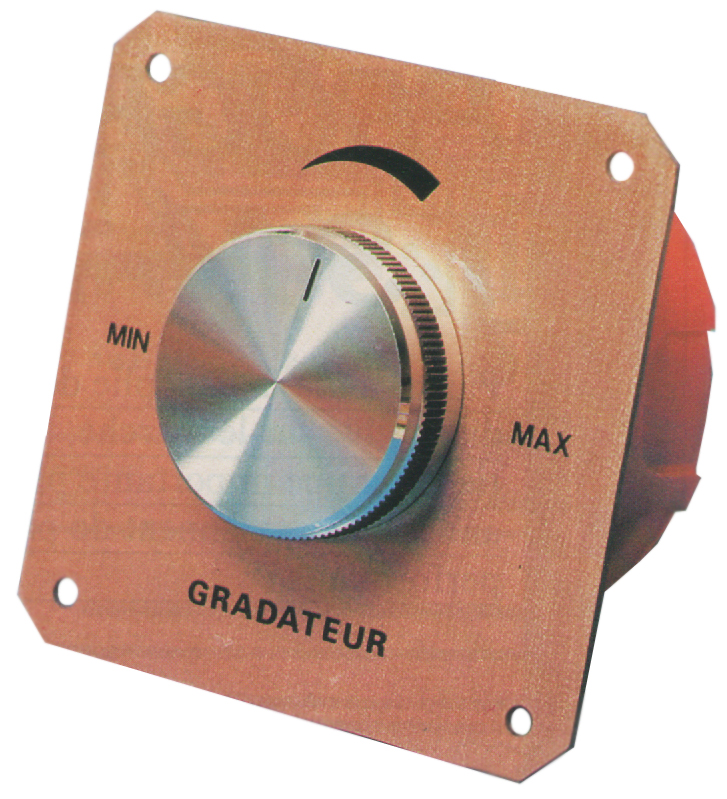
\includegraphics[width=\textwidth]{Gradateur_lumiere_mural}
\end{center}
\end{minipage}

\begin{minipage}{0.46\textwidth}
Dans ce TP, nous allons mixer toutes les couleurs d'une LED RGB.
\end{minipage}\hfill
\begin{minipage}{0.46\textwidth}
\begin{center}
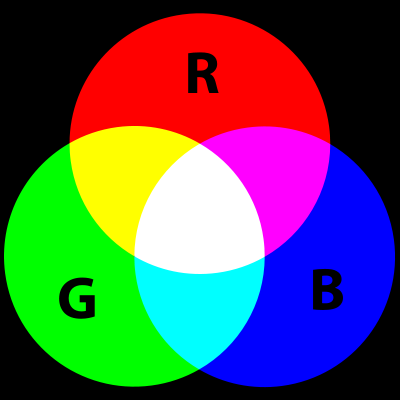
\includegraphics[width=\textwidth]{rgb_color}
\end{center}
\end{minipage}


\begin{center}
\end{center}

\question Quelles sont les trois couleurs des trois types de cônes de la rétine humaine ?
\reponse

\question Pour que l'oeuil humain voit la couleur blanche, quels cônes faut'il exciter ?
\reponse

\question Pour que l'oeuil humain voit la couleur jaune, quels cônes faut'il exciter ?
\reponse

\question Dans un écran, chaque pixel est composé de trois couleurs. Lesquelles ?
\reponse

\question De quoi sont composées les couleurs blanches et noires ?
\reponse
\reponse
%}}}

\bigskip

\partie{Principe du gradateur}\\ %{{{1
La PWM, abréviation de Pulse Width Modulation\footnote{modulation de la largeur d'impulsion}, est une technique utilisée pour coder le niveau du signal analogique en signaux numériques. Un ordinateur ne peut pas fournir de tension analogique : il ne peut seulement fournir des valeurs de tensions numériques telles que 0V ou 5V (et aucune autres valeurs).

Pour pour coder un niveau de signal analogique précis, le principe consiste à moduler le rapport cyclique des impulsions PMW.

\begin{figure}[!h]
\begin{center}
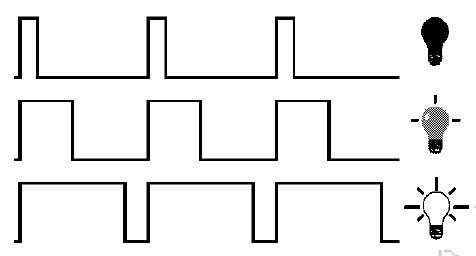
\includegraphics[width=.49\textwidth]{PWM_lampes}\hfill
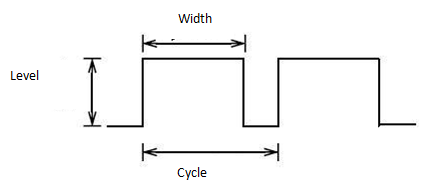
\includegraphics[width=.49\textwidth]{PWM_keywords}\\
\caption{Principe géréral la modulation de largeur d'impulsion, ou Pulse Wave Modulation. La largeur de l'impulsion est simplement la largeur du créneau sur la figure, elle est exprimé en seconde. Le rapport cyclique est lui sans unité et varie entre 0 et 1. Il représente la fraction de temps où la tension est à sa valeur haute. Si le signal est la moitié du temps à la valeur haute, le rapport cyclique vaut 0,5. S'il est tout le temps haut, il vaut 1. Il vaut 0 s'il est tout le temps bas.}
\label{PWM}
\end{center}
\end{figure}

\question Dans la figure \ref{PWM}, combien d'impulsions sont représentées pour les trois cas de figures ?
\reponse

\question Est-ce que les impulsions ont lieu à la même fréquence ?
\reponse

\question Quel est le lien (l'équation) entre la fréquence et la période (ou le cycle) d'un signal ?
\reponse

\question Quel paramètre de l'impulsion varie entre chaque cas de figure ? S'aider de la terminologie du titre de la figure pour répondre.
\reponse

\question Si la largeur d'impulsion est nulle, c'est à dire qu'elle fait 0\% du cycle, la tension délivrée est constamment à 0V. Celà revient à appliquer une tension continue de 0 V. \\Si la largeur de l'impulsion fait 100\% du cycle, comment est la tension de sortie ? Quelle tension cela revient-il à appliquer ?
\reponse
\reponse

\question En principe, un simple composant permet de hacher ainsi la tension. Lequel ?
\reponse

La valeur de la tension de sortie est calculée via le temps d'activation et de désactivation. Tension de sortie = (temps d'activation / temps d'impulsion) * valeur de tension maximale.
\begin{equation*}
V_{OUT}= \frac{T_{ON}}{T_{cycle}} \cdot V_{IN}
\end{equation*}

\begin{figure}[!h]
\begin{center}
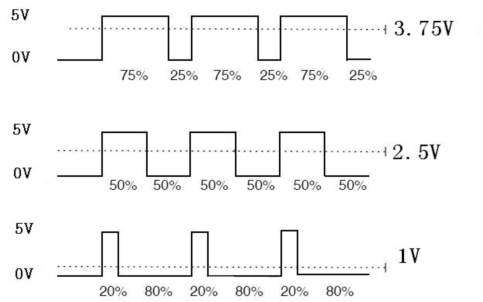
\includegraphics[width=.75\textwidth]{PWM_voltage}
\caption{Principe géréral la modulation de largeur d'impulsion, ou Pulse Wave Modulation.}
\label{PWM}
\end{center}
\end{figure}

\question Retrouver l'application numérique qui a permis de calculer que la tension de sortie valait 3,75 Volt dans le premier cas de figure.
\reponse

\question Retrouver l'application numérique qui a permis de calculer que la tension de sortie valait 2,5 Volt dans le deuxième cas de figure.
\reponse

\question Retrouver l'application numérique qui a permis de calculer que la tension de sortie valait 1 Volt dans le troisième cas de figure
\reponse

\question Le microcontrolleur de la carte arduino UNO permet de générer 6 PWM. Sur quelles broches de la carte sont elles branchées ?
\reponse

\question Réaliser le montage de la figure \ref{CablageGradateur}.

\begin{figure}[!h]
\begin{center}
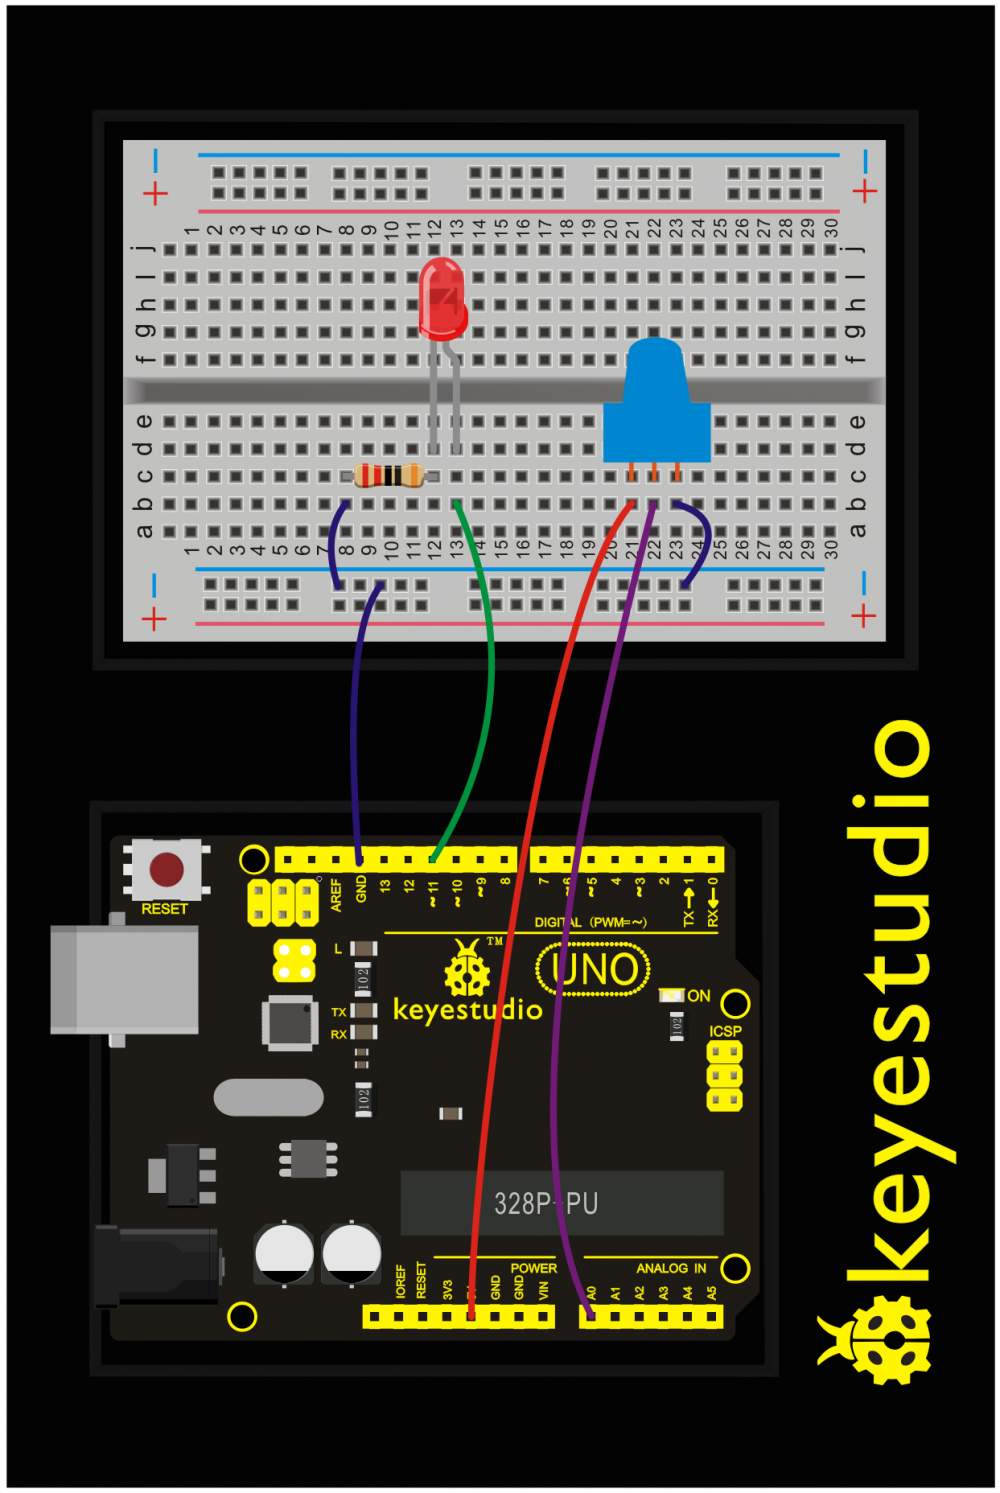
\includegraphics[height=1\textwidth,angle=270]{cablage_gradateur}
\caption{Montage à réaliser pour tester le fonctionnement en gradateur}
\label{CablageGradateur}
\end{center}
\end{figure}

\question Implémenter le code suivant :
\begin{lstlisting}
int potpin=0;  // initialize analog pin 0
int ledpin=11; // initialize digital pin 11 (PWM output)
int val=0;     // Temporarily store variables' value from the sensor

void setup() {
    // define digital pin 11 as "output"
    pinMode(ledpin,OUTPUT);
    // set baud rate at 9600
    Serial.begin(9600);
    // attention: for analog ports, they are automatically set up as "input"
    }

void loop() {
    // read the analog value from the sensor and assign it to val
    val=analogRead(potpin);
    // display value of val
    Serial.println(val);
    // turn on LED and set up brightness (maximum output of PWM is 255)
    analogWrite(ledpin,val/4);
    // wait for 0.01 second
    delay(10);
    }
\end{lstlisting}

\tcbox{\textbf{Constatation professeur :} \hspace{5cm} } % package tcolorbox

\question Quelle est la fonction de la pin 0 ?
\reponse

\question Quelle est la fonction de la pin 11 ?
\reponse

\question Lors que la tension appliquée à la pin \texttt{potpin} est 0V, quelle est la valeur retournée par la fonction \texttt{analogRead(potpin)}; ? \footnote{Comme le codage est 8 bits, les valeurs à la sortie du convertisseur analogique  numérique sont comprises en 0 et $2^8-1=1023$}
\reponse

\question Lors que la tension appliquée à la pin \texttt{potpin} est 5V, quelle est la valeur retournée par la fonction \texttt{analogRead(potpin)}; ?
\reponse

\question Lors que la tension appliquée à la pin \texttt{potpin} est 2,5V, quelle est la valeur retournée par la fonction \texttt{analogRead(potpin)}; ?
\reponse

\question Un potentiomètre est un bel exemple d'un circuit branchant deux résitances en série. Quel est le nom de ce montage ? Quel est la formule associée à ce montage ?
\reponse
\reponse

\question Ainsi, pour avoir 2,5V au point milieu d'un potentiomètre dont la résistance totale est de 10 k$\Omega$, quel doivent être les valeurs des deux résistances ? Vérifez le résultat grâce à la formule ci-dessus.
\reponse
\reponse

\question Ainsi, pour avoir 1V au point milieu d'un potentiomètre dont la résistance totale est de 10 k$\Omega$, quel doivent être les valeurs des deux résistances ? Vérifez le résultat grâce à la formule ci-dessus.
\reponse
\reponse

\question Ouvrez le terminal série de l'environnement arduino et observez la valeur \texttt{val} évoluer alors que vous faites varier le potentiomètre. Prennez un multimètre et vérifier que la valeur mesurée codée sur 8 bits correspond à la valeur mesurée avec un volmètre (pour deux ou trois valeurs). Précisez le calcul de la conversion analogique numérique dans les lignes ci-dessous pour deux réglages différents du potentiomètre.
\reponse
\reponse
\reponse
\reponse
%}}}

\newpage

\partie{Trois gradateurs pour 3 couleurs} \\ %{{{1

\question Réaliser le circuit la figure \ref{MontageTroisCouleurs}. \\


\begin{figure}[!ht]
\begin{center}
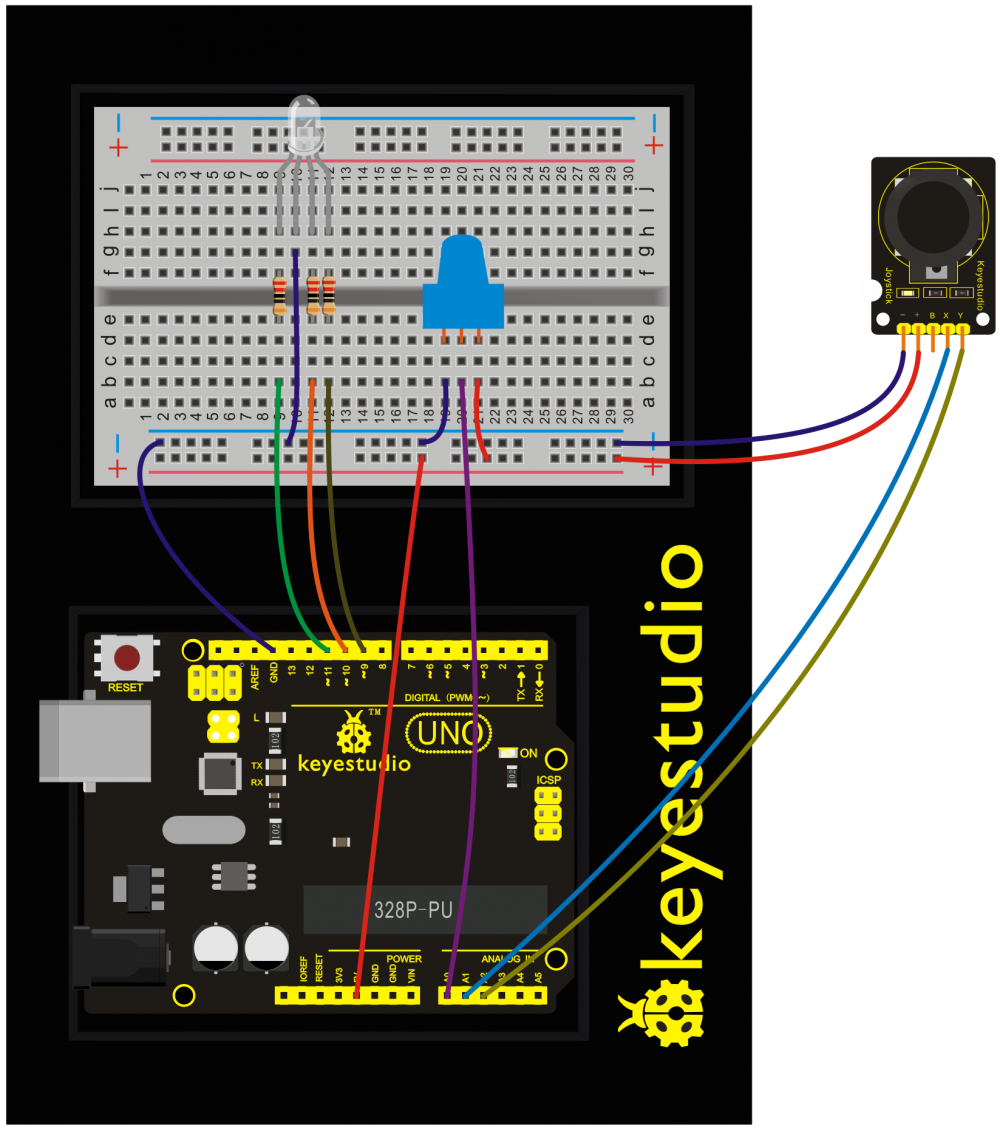
\includegraphics[height=\textwidth,angle=270]{montage_3couleurs}\\
\caption{Montage à réaliser pour varier la couleur émise d'une LED RGB.}
\label{MontageTroisCouleurs}
\end{center}
\end{figure}


\question Implémenter le code suivant et tester le montage. Une meilleure apréciation de la couleur est obtenue en mettant une feuille de papier blanc juste au dessus de la LED.  \\
\begin{lstlisting}
int redpin = 11;
int greenpin =10;
int bluepin =9;

int value1;
int value2;
int value3;

void setup() {
  pinMode(redpin, OUTPUT);
  pinMode(bluepin, OUTPUT);
  pinMode(greenpin, OUTPUT);
  Serial.begin(9600);
}

void loop() {
  value1=map( analogRead(0),0,1023,0,255);
  value2=map( analogRead(1),0,1023,0,255);
  value3=map( analogRead(2),0,1023,0,255);
  analogWrite(11, value1);
  Serial.print("value1= ");
  Serial.println(value1);
  delay(100);
  analogWrite(10, value2);
  Serial.print("value2= ");
  Serial.println(value2);
  delay(100);
  analogWrite(9, value3);
  Serial.print("value3= ");
  Serial.println(value3);
  delay(100);
}
\end{lstlisting}

\tcbox{\textbf{Constatation professeur :} \hspace{5cm} } % package tcolorbox

\question Que fait la fonction map() ? \footnote{Trouver la ducumentation officielle de cette fonction et recopier la description}
\reponse
\reponse
\reponse

\question Quelles entrées du programme sont lues ? Avec quelles fonctions ?
\reponse
\reponse
\reponse
\reponse

\question Quelles sorties sont écrites ? Avec quelles fonctions ?
\reponse
\reponse
\reponse
\reponse

\question Quelles valeurs sont lues sur le terminal arduino pour obtenir du jaune ?
\reponse

\question Quelles valeurs sont lues sur le terminal arduino pour obtenir du magenta ?
\reponse

\question Quelles valeurs sont lues sur le terminal arduino pour obtenir du cyan ?
\reponse

\question Comment obtenir du jaune de plus faible intensité ?
\reponse

\question Plutot que d'avoir du mal avec les potentiomètres pour avoir exactement la couleur désirée, que pouvez-vous plutôt faire ?
\reponse

\question Implémentez l'idée décrite ci-dessous et écrivez ci-dessous les lignes du code source que vous avez ajouté :
\reponse
\reponse
\reponse
\reponse
\tcbox{\textbf{Constatation professeur :} \hspace{5cm} } % package tcolorbox

%}}}



\end{document}

% vim:fdl=0 : wrap

